\documentclass{article}
\usepackage{parskip}
\usepackage{caption}
\usepackage{subcaption}
\usepackage{multirow}

% Language setting
% Replace 'english' with e.g. 'spanish' to change the document language
\usepackage[italian]{babel}

\addto\captionsenglish{\renewcommand{\figurename}{Figura}}

% Set page size and margins
% Replace 'letterpaper' with 'a4paper' for UK/EU standard size
\usepackage[letterpaper,top=2cm,bottom=2cm,left=3cm,right=3cm,marginparwidth=1.75cm]{geometry}

% Useful packages
\usepackage{amsmath}
\usepackage{graphicx}
\graphicspath{ {./images/} }
\usepackage[colorlinks=true, allcolors=blue]{hyperref}


\usepackage{listings}
\usepackage{xcolor}

\definecolor{codegreen}{rgb}{0,0.6,0}
\definecolor{codegray}{rgb}{0.5,0.5,0.5}
\definecolor{codepurple}{rgb}{0.58,0,0.82}
\definecolor{backcolour}{rgb}{0.95,0.95,0.92}

\lstdefinestyle{mystyle}{
    backgroundcolor=\color{backcolour},   
    commentstyle=\color{codegreen},
    keywordstyle=\color{magenta},
    numberstyle=\tiny\color{codegray},
    stringstyle=\color{codepurple},
    basicstyle=\ttfamily\footnotesize,
    breakatwhitespace=false,         
    breaklines=true,                 
    captionpos=b,                    
    keepspaces=true,                 
    numbers=left,                    
    numbersep=5pt,                  
    showspaces=false,                
    showstringspaces=false,
    showtabs=false,                  
    tabsize=2
}

\lstset{style=mystyle}

\begin{document}

\begin{center}
    {\Large Alma Mater Studiorum - Università di Bologna}
    
    \vspace{0.5cm}
    {\bf \large Relazione per il corso di Data Science}
\end{center} 

\noindent
{ Liam Cavini} \hfill {\bf 2° Foglio, Ottimizzazione}\\
{\ Semestre Invernale 2024/2025} \hfill 23/10/2024



\subsection*{Esercizio 1 - Ottimizzazione non vincolata}
\textbf{(a)} Per trovare i minimi della funzione:
\[
f(x, y) = x^2  - 2x  + x^2 y^2 - 2xy
\]

si calcola il gradiente e si trovano i punti critici. Si studia successivamente se la hessiana valutata in questi punti è definita o semidefinita positiva. Si trova così che i punti critici sono $(1,1)$ e $(0,-1)$, e che il primo di questi corrisponde ad un minimo locale ed il secondo ad un punto di sella.

Partendo da $(0,0)$ il metodo della discesa del gradiente (con tasso di apprendimento $\alpha = 0.2$) trova il minimo senza problemi, come si può osservare in Figura \ref{fig:countour_plot}.

Il metodo di Newton invece in questo caso fallisce, in un solo step infatti raggiunge il punto di sella, come mostrato sempre in Figura \ref{fig:countour_plot}. Se si calcola la hessiana esplicitamente nel punto $(0,0)$ si trova che: 
\[
H(0,0) =
\begin{bmatrix}
    0 && -0.5 \\
    -0.5 && -0.5 \\
\end{bmatrix}
\]
Moltiplicando la hessiana per il gradiente in $(0,0)$ (il quale risulta essere $(-2, 0)$), si osserva infatti che il metodo di Newton non aggiorna il parametro $x$ nella prima iterazione, aggiornando invece $y$ ad un valore più piccolo, allontanandosi di conseguenza minimo.

\begin{figure}[htbp]
     \centering
     \begin{subfigure}{.49\textwidth}
        \centering
        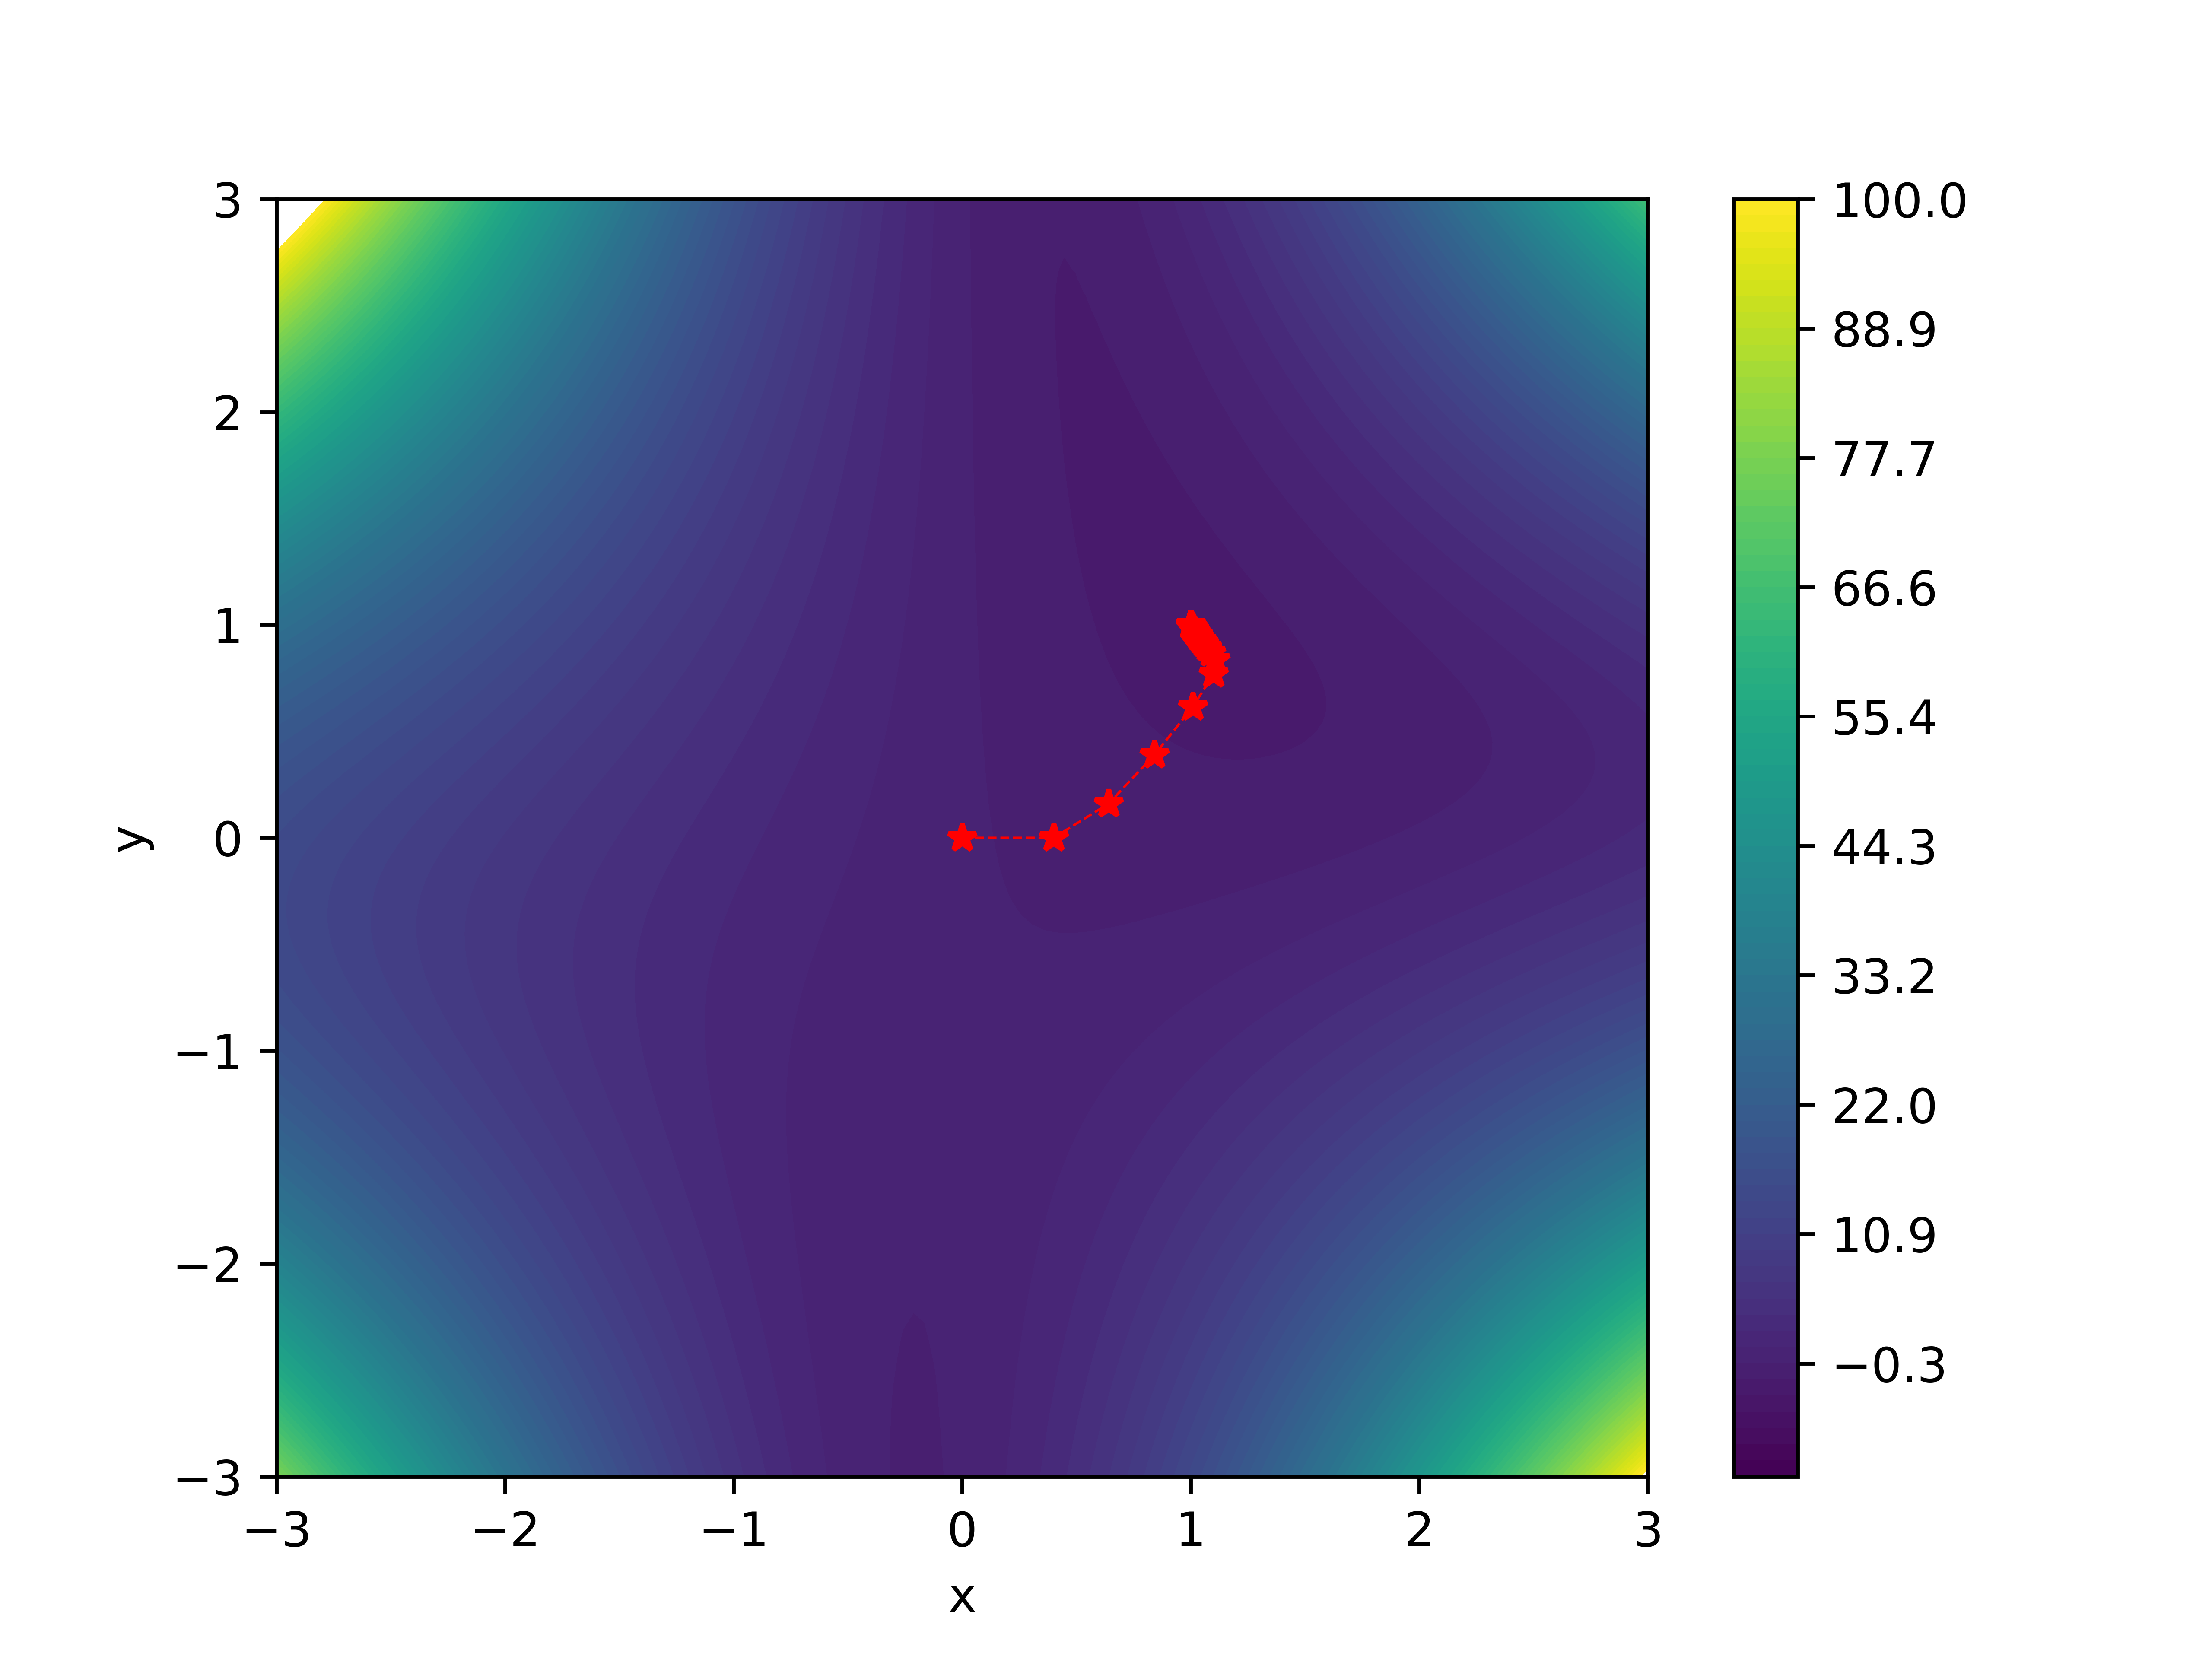
\includegraphics[width=1 \textwidth]{images/gradient_descent.png}
     \end{subfigure}
     \begin{subfigure}{.49\textwidth}
        \centering
        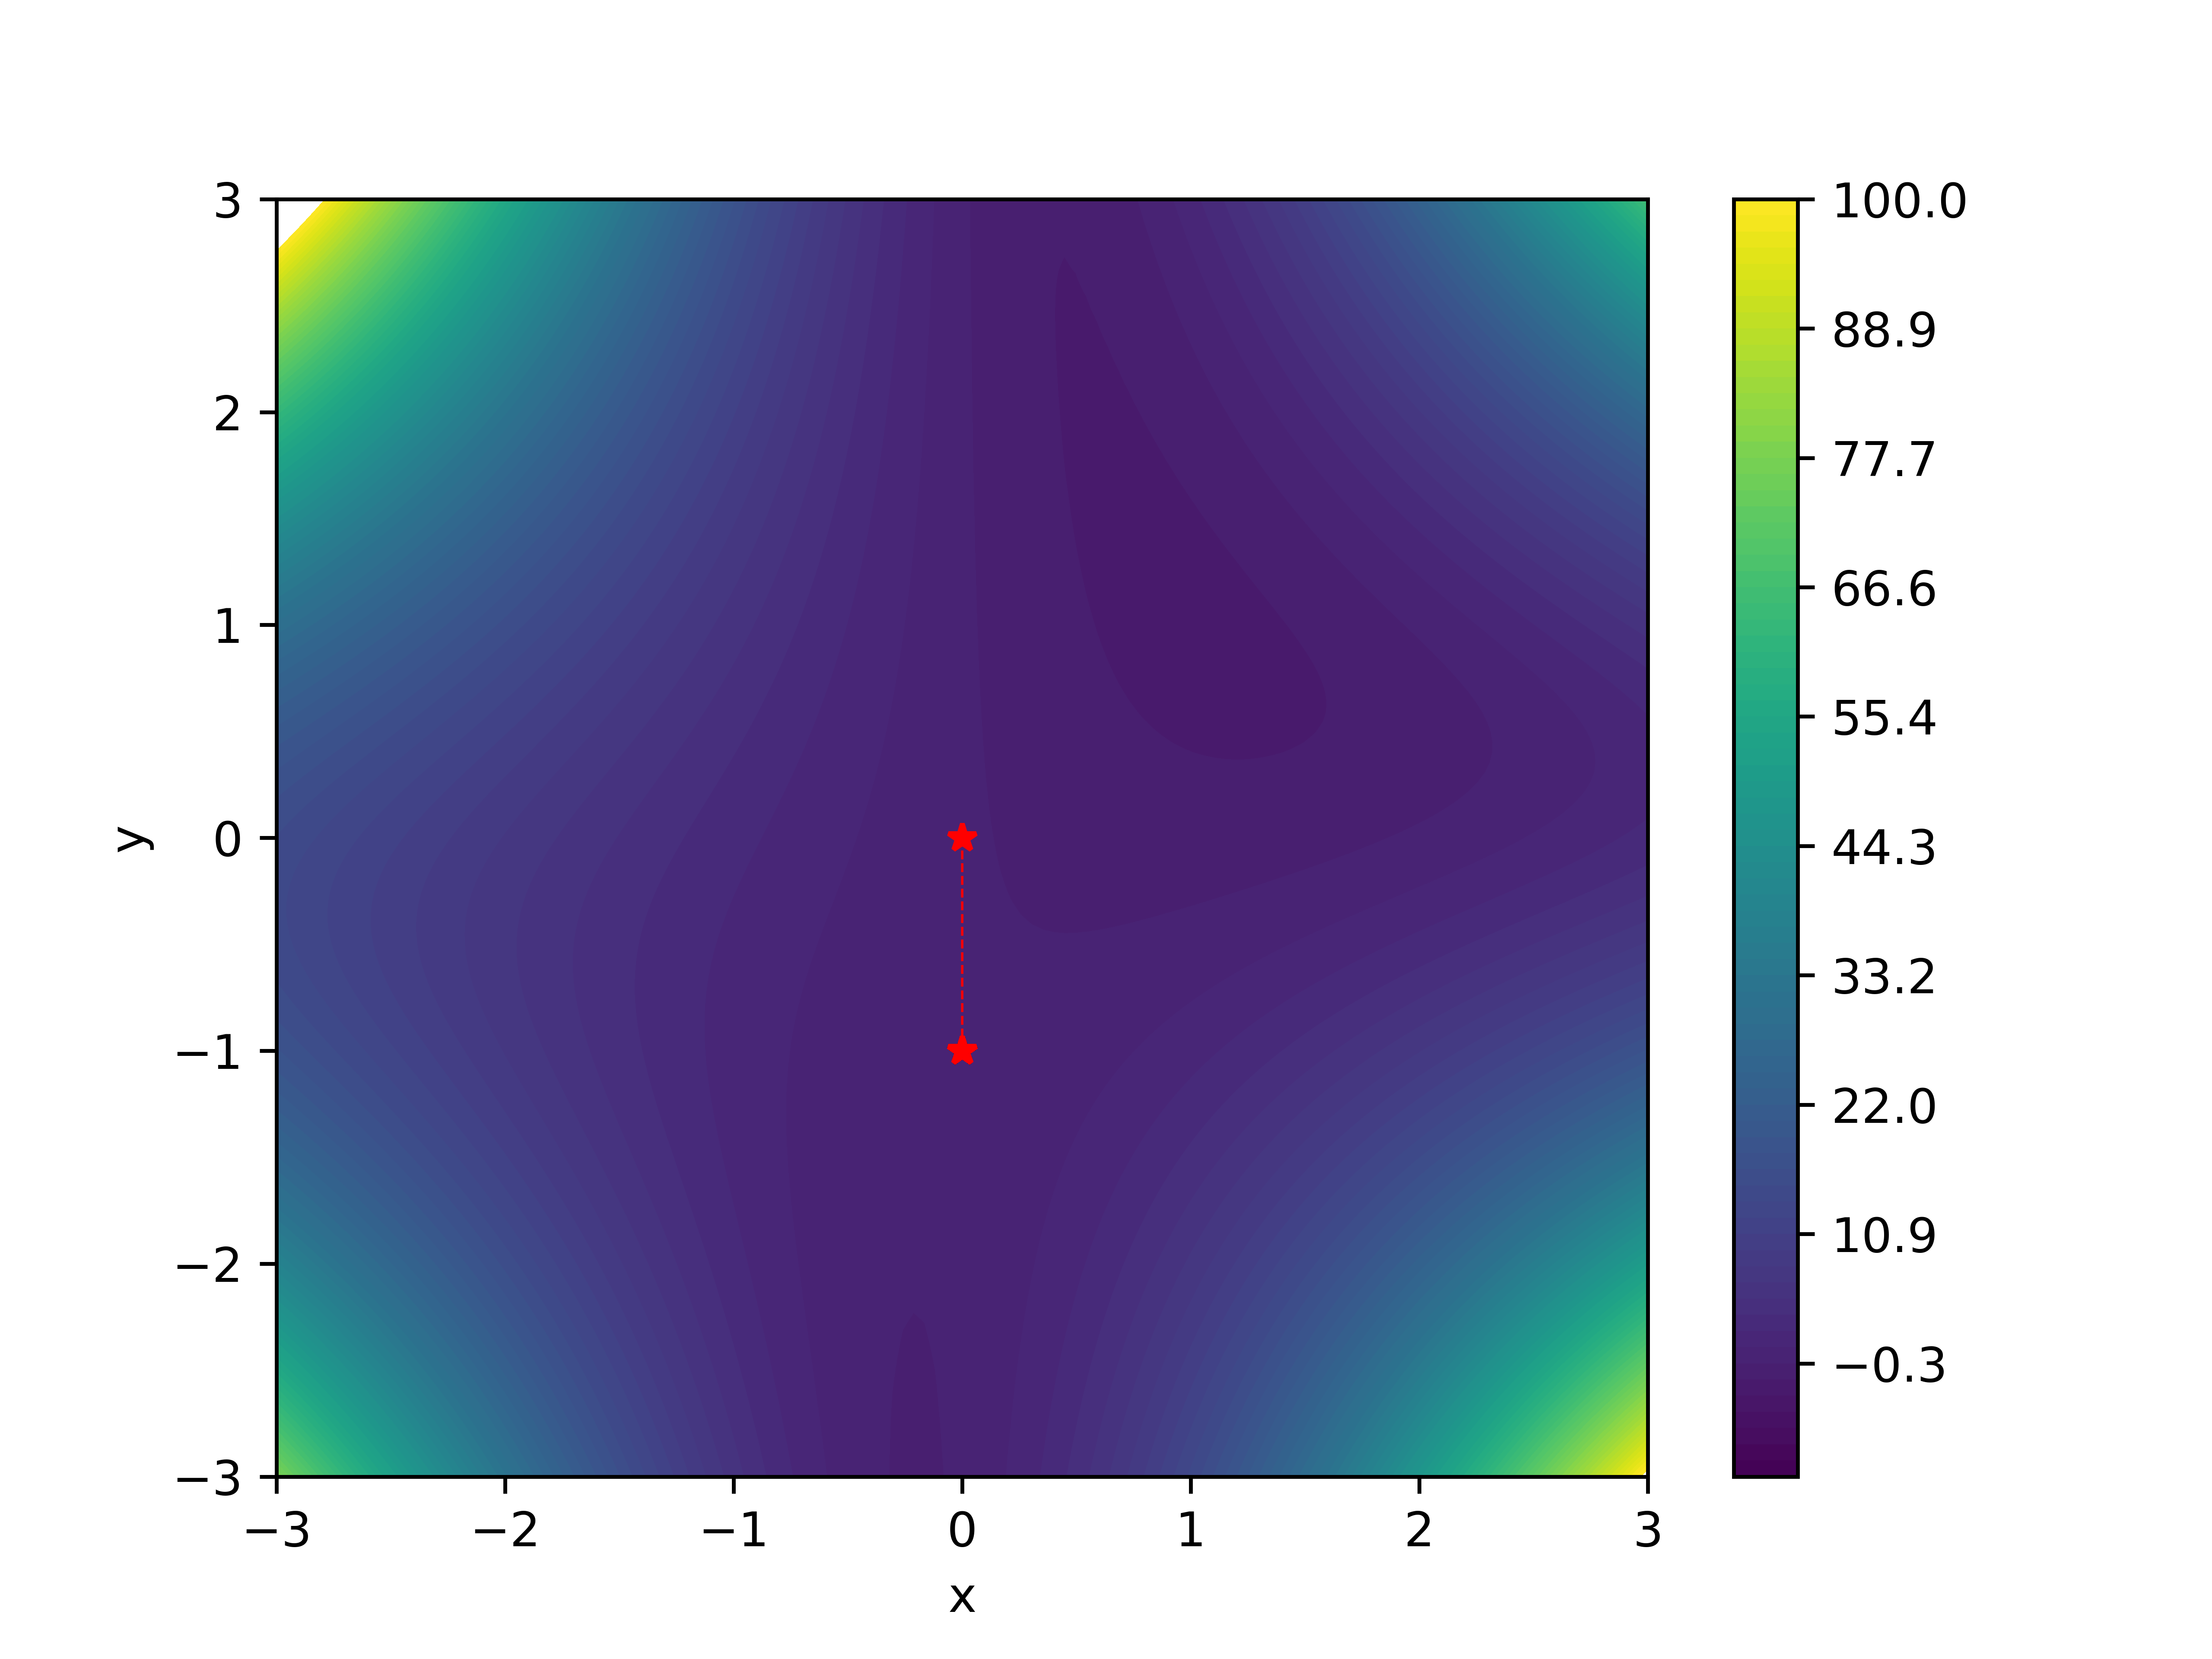
\includegraphics[width=1\textwidth]{images/newton_method.png}
    \end{subfigure} 
    %todo: migliorare caption
    \caption{\emph{Le immagini mostrano una planimetria della funzione. I tratti rossi indicano il percorso compiuto dalla discesa del gradiente che inizia dal punto $(0,0)$. A sinisitra abbiamo il risultato ottenuto con il metodo classico, con tasso di apprendimento pari a $0.2$, che raggiunge il minimo globale. A destra il risultato ottenuto col metodo di Newton, che si ferma sul punto di sella.}}
    \label{fig:countour_plot}
\end{figure}

Il codice usato per la discesa del gradiente è il seguente:

\begin{lstlisting}[language = Python]
import numpy as np
import matplotlib.pyplot as plt

def gradient(pos):
    x = pos[0]
    y = pos[1]
    return np.array([2*x-2+2*x*y**2-2*y, 2*x**2*y -2*x])

def update(pos, learning_rate):
    pos -= learning_rate * gradient(pos)

iteration_number = 10000
inital_pos = np.array([0,0])
positions = np.zeros((iteration_number+1,2))
positions[0] = inital_pos

learning_rate = 0.2

for i in range(iteration_number):
    positions[i+1] = positions[i]
    update(positions[i+1], learning_rate)

#matplotlib
X, Y = np.meshgrid(np.linspace(-3, 3, 128), np.linspace(-3, 3, 128))
Z = X**2 - 2*X  + X**2 * Y**2 - 2*X*Y

fig, axs = plt.subplots()
co = axs.contourf(X, Y, Z, levels=np.linspace(-10, 100, 80))
fig.colorbar(co, ax=axs)

def overlay_trajectory_contour(axs,trajectory, label,color='k',lw=2):
    xs=trajectory[:,0]
    ys=trajectory[:,1]
    axs.plot(xs,ys, color, label=label,lw=lw)
    return axs;

overlay_trajectory_contour(axs,positions,'$\eta=$%s'% learning_rate,'r--*', lw=0.5)
\end{lstlisting}
Mentre per il metodo di Newton si è usato lo stesso codice, sostituendo al learning rate l'inversa della matrice hessiana valutata con gli attuali parametri. Si riporta sotto solo lo spezzone di codice modificato:

\begin{lstlisting}[language = Python]
#[...] previous code goes here
def update(pos, learning_rate):
    pos -= learning_rate @ gradient(pos)

def hess_inv(pos):
    x = pos[0]
    y = pos[1]
    hessian = np.array([[2+2*y**2, 4*x*y-2],[4*x*y-2, 2*x**2]])
    return np.linalg.inv(hessian)

#[...] previous code goes here
for i in range(iteration_number):
    positions[i+1] = positions[i]
    update(positions[i+1], hess_inv(positions[i]))

#[...] previous code goes here
\end{lstlisting}

\subsection* {Esercizio 2 - Metodi di discesa del gradiente}
\textbf{(a)} 
L'esercizio consiste nell'eseguire il fit di dati generati dalla funzione $\sin(2\pi x)$, con l'aggiunta di rumore, implementando una regressione polinomiale tramite discesa del gradiente stocastica.

La Figura \ref{fig:sin_fit} mostra il risultato del fit usando un polinomio di grado 9 (quindi 10 parametri), un learning rate di 0.2 e un batch size di 20. Questo è stato comparato al risultato ottenuto tramite l'espansione di Taylor (sempre di grado 9) di $\sin(2 \pi x)$ intorno al punto $0.5$. 

Il fit, nonostante sia graficamente simile al risultato ottenuto con l'espansione, risulta avere dei coefficienti polinomiali che differiscono di ordini di grandezza, e talvolta di segno, da quelli della serie di Taylor.

\begin{figure}[htbp]
     \centering
     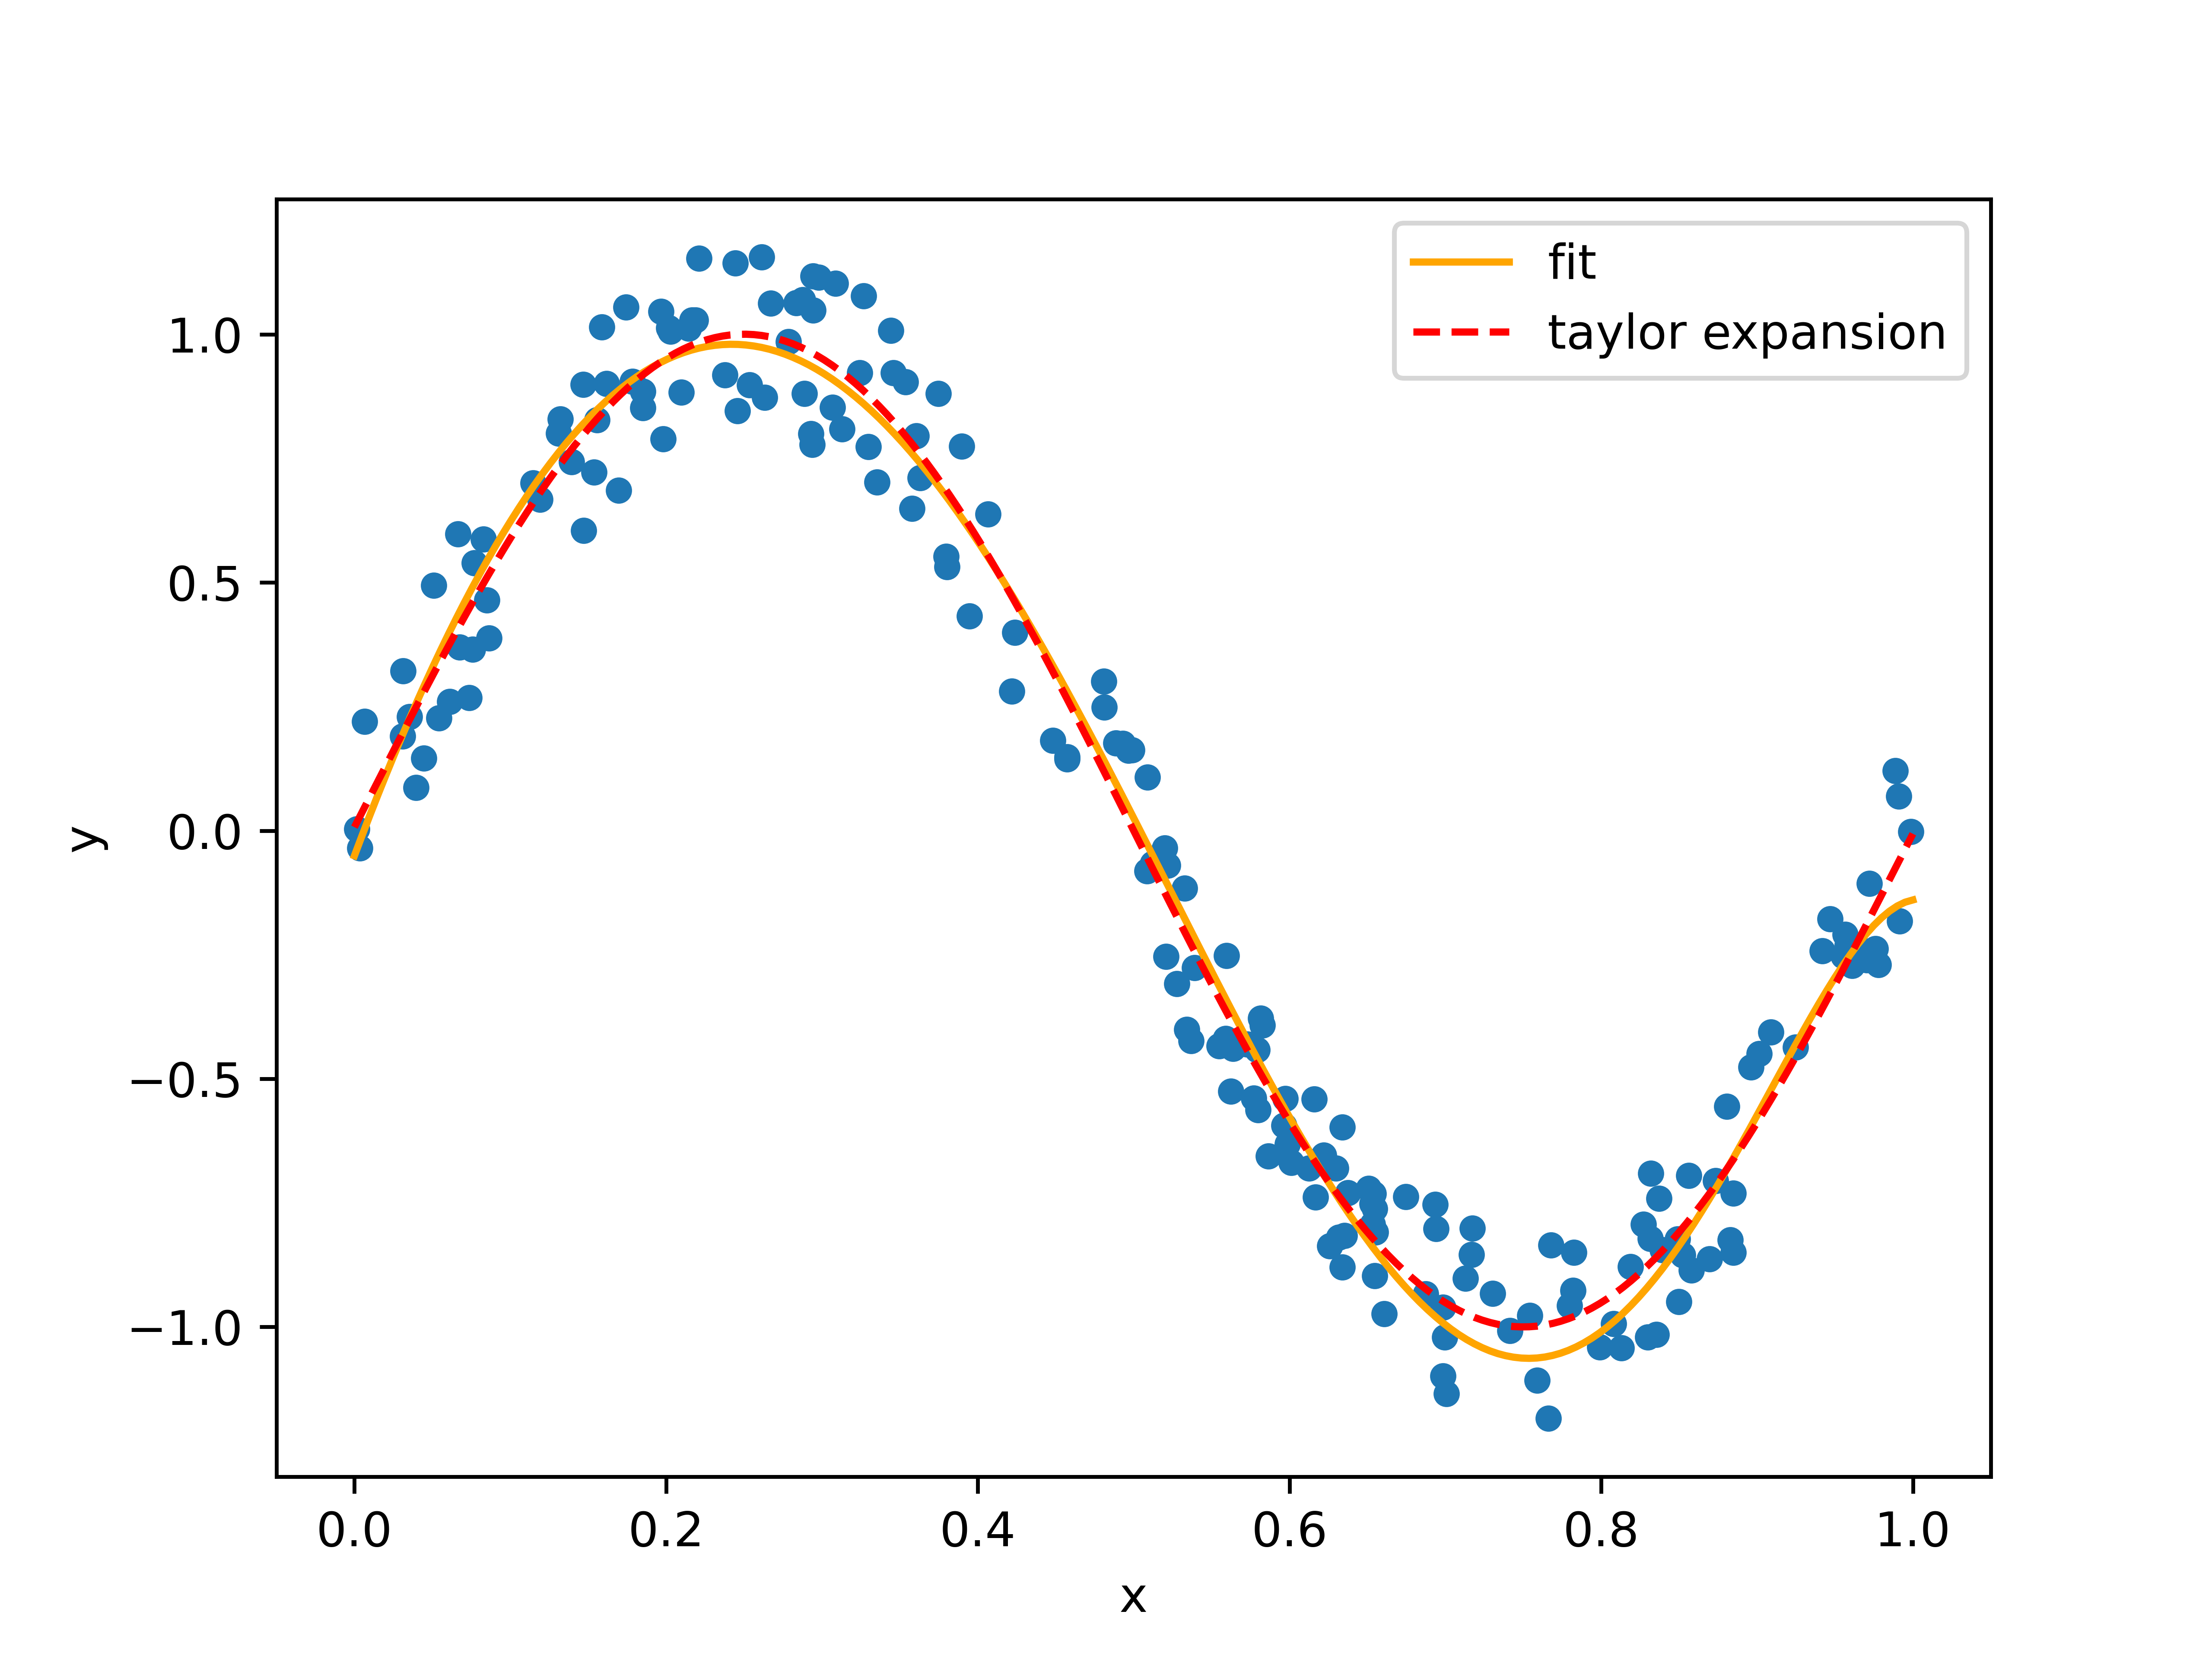
\includegraphics[width = 0.6\textwidth]{./../images/sine_fit.png}
    %todo: migliorare caption
    \caption{\emph{In blu i data points generati, in arancione la curva ottenuta da un fit lineare dei coefficienti di un polinomio di ordine $9$, in rosso l'espansione di Taylor intorno a $0.5$ (sempre al nono ordine).}}
    \label{fig:sin_fit}
\end{figure}

Si riporta sotto il codice python utilizzato:
\begin{lstlisting}[language = python]
#number of data
n_data = 200
iteration_number = 100000
learning_rate = 0.2
batch_size = 20
# pol_order is the order of the polynomial -1
pol_order = 10

x = np.random.rand(n_data)

y = np.sin(2*np.pi*x)+(np.random.rand(len(x))-0.5)*(0.2/0.5)

fig, ax = plt.subplots()
ax.scatter(x,y, s = 20)

parameters = np.random.rand(pol_order)-0.5

def batch(x,y, batch_size):
    in_batch = np.random.choice(np.arange(len(x)), batch_size)
    x_batch = np.array([x[i] for i in in_batch])
    y_batch = np.array([y[i] for i in in_batch])
    return (np.array(x_batch), np.array(y_batch))

def polynomial(parameters, x, order):
    temp = np.zeros(len(x))
    for i in range(order):
        temp += parameters[i]*(x**i)
    return temp

def gradient(parameters, x, y):
    temp = np.zeros(len(parameters))
    pol = polynomial(parameters, x, len(parameters))
    for i in range(0, len(parameters)):
        temp[i] = -2*np.sum((y-pol)*(x**i))/len(x)
    return temp

def update(parameters, learning_rate, x, y):
    parameters -= learning_rate * gradient(parameters, x , y)


for i in range(iteration_number):
    batch_x, batch_y = batch(x,y, batch_size)
    update(parameters, learning_rate, batch_x ,batch_y)

x_lin = np.linspace(0., 1., n_data)
y_predicted = polynomial(parameters, x_lin ,pol_order)
ax.plot(x_lin, y_predicted, color = 'orange', label = "fit")

#comparing with taylor expansion
par_taylor = np.array([0.00692527, 6.13253, 1.4848, -50.0794, 34.0311, -10.1117, 173.146, \
-301.822, 189.264, -42.0587, -3.23628*10**(-15)])
y_taylor = polynomial(par_taylor[:pol_order], x_lin, pol_order)

ax.plot(x_lin, y_taylor, color = 'red', linestyle = 'dashed', label = "taylor expansion")

ax.legend()
\end{lstlisting}

\textbf{(b)} Si è ottimizzata la funzione:
\[
f(x) = x^4 - 3x^3 +2
\]
usando la discesa del gradiente, la discesa del gradiente con momento e la discesa del gradiente accelerata di Nesterov.
Un semplice studio della funzione mostra che questa ha il minimo globale in $x = \frac{9}{4}$ e un punto di sella in $x = 0$. 

La Tabella \ref{tab:dati} mostra la performance dei vari algoritmi al variare dei parametri. Nei casi riportati nella prima e nelle ultime due righe della tabella, la prestazione dei due algoritmi più sofisticati risulta migliore di quella ottenuta dalla discesa del gradiente classica. 
L'argoritmo classico risulta essere più lento poiché considera solamente il gradiente nella posizione attuale (che vicino ai punti critici è prossimo a zero), mentre quelli più avanzati tengono conto della elevata pendenza iniziale.


\begin{table}[htb]
    \centering
    \begin{tabular}[]{|c|c|c|c|c|c|}
        \hline
        $x_0$ & $\alpha$ & $\gamma$ & $n$ gradient descent & $n$ momentum & $n$ Nesterov\\
        \hline
        8 & 0.001 & 0.05 & 212 & 201 & 201\\
        8 & 0.001 & 0.5 & 212 & 82 & 98\\
        8 &  0.001 & 0.8 & 212 & 1204 (sella) & 2140 (sella)\\
        -8 & 0.001 & 0.5 & 10000+ (sella) & 5318 (sella) & 5400 (sella)\\
        -8 & 0.001 & 0.8 & 10000+ (sella) & 129 & 55\\
        \hline
    \end{tabular}
\caption{\emph{La tabella mostra la performance dei vari algoritmi al variare dei parametri rilevanti.
$x_0$ indica la posizione iniziale, $\alpha$ il tasso di apprendimento, $\gamma$ il momentum parameter, ed $n$ il numero di iterazioni che impiega un determinato algoritmo a raggiungere la destinazione.
In caso quest'ultima non fosse il minimo ma il punto di sella, al valore numerico di $n$ viene accostato un \emph{(sella)}. Se al valore numerico è invece accostato il simbolo $+$,
allora l'algoritmo raggiunge la destinazione, ma si avvicina talmente lentamente da non raggiungerla nel numero di iterazioni che compie.}}
\label{tab:dati}
\end{table}

Nell'ultimo caso riportato in Tabella \ref{tab:dati} l'algoritmo classico raggiunge il punto di sella, mentre i due algoritmi più avanzati superano questo per poi oscillare intorno al minimo globale.
Questo comportamento è mostrato in Figura \ref{fig:confronto_algoritmi}, ed è sempre spiegabile considerando la ``memoria" che gli algoritmi più avanzati possiedono della derivata nella posizione iniziale.

L'algoritmo classico invece mostra una migliore performance nel caso riportato nella terza riga della Tabella \ref{tab:dati}.
Stavolta gli algoritmi più avanzati saltano il minimo globale, per invece oscillare intorno al punto di sella.

\begin{figure}[!htb]
    \centering
    \begin{subfigure}{.49\textwidth}
       \centering
       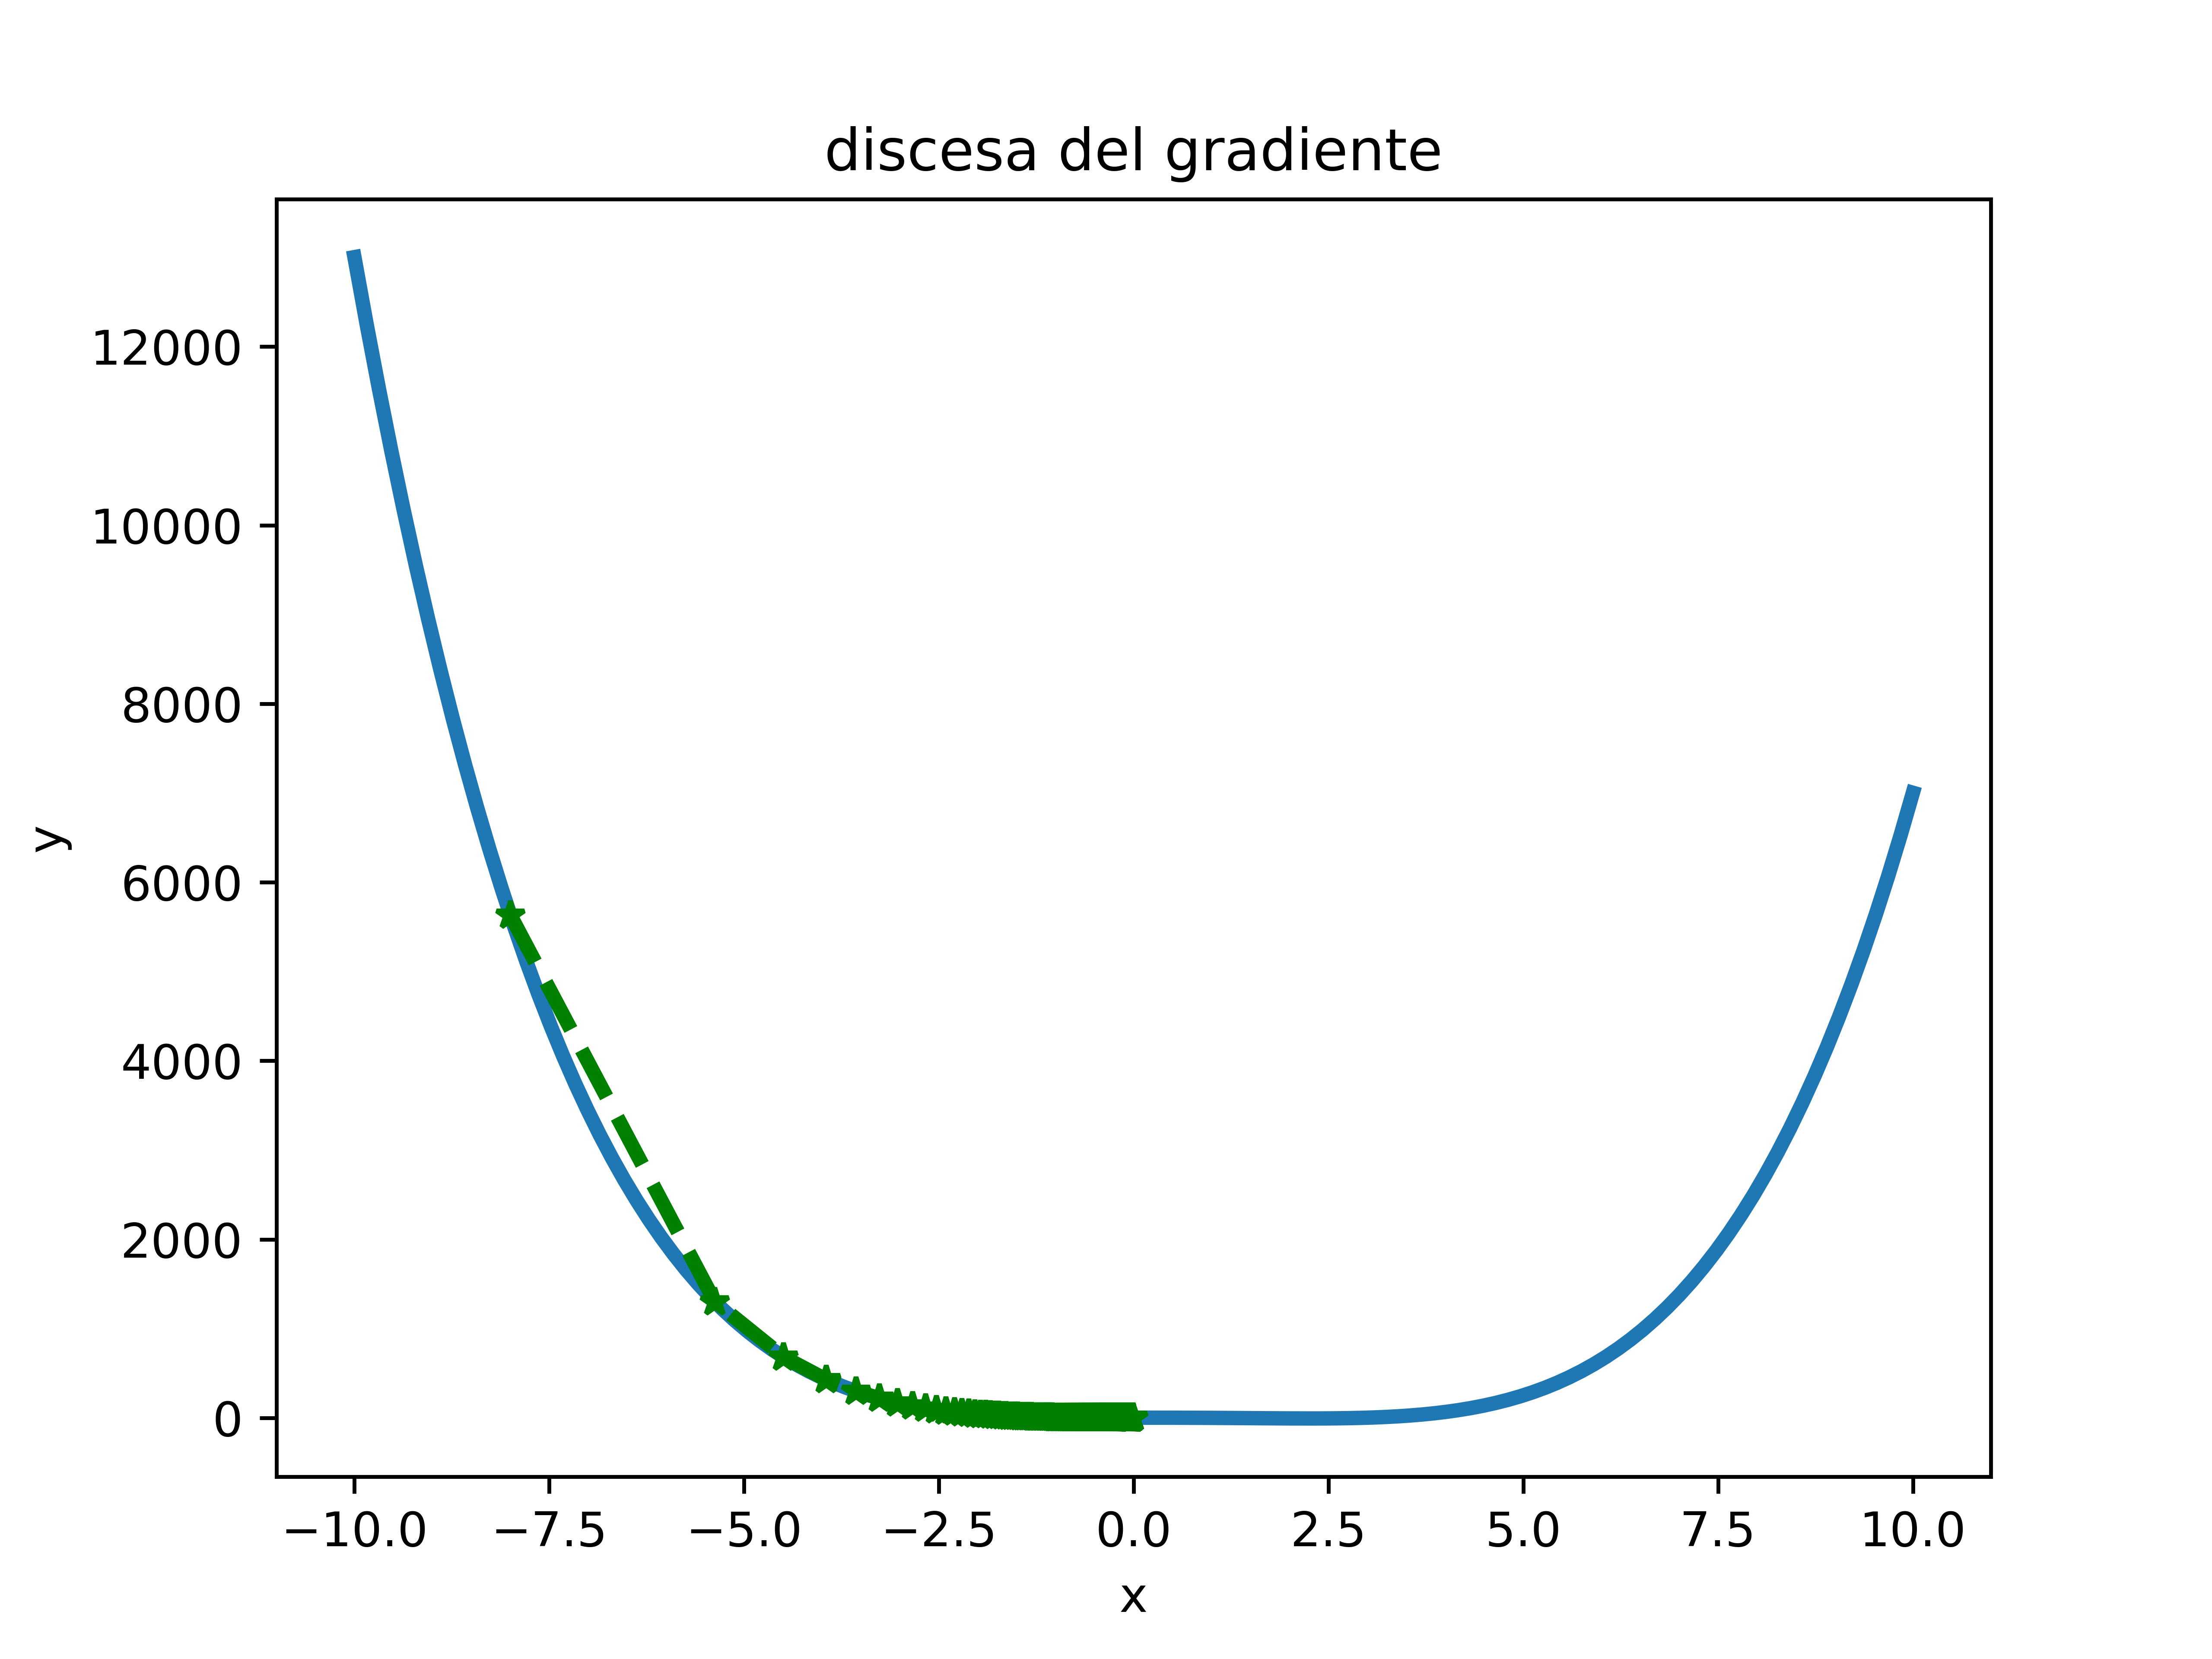
\includegraphics[width=1 \textwidth]{images/classico.png}
    \end{subfigure}
    \begin{subfigure}{.49\textwidth}
       \centering
       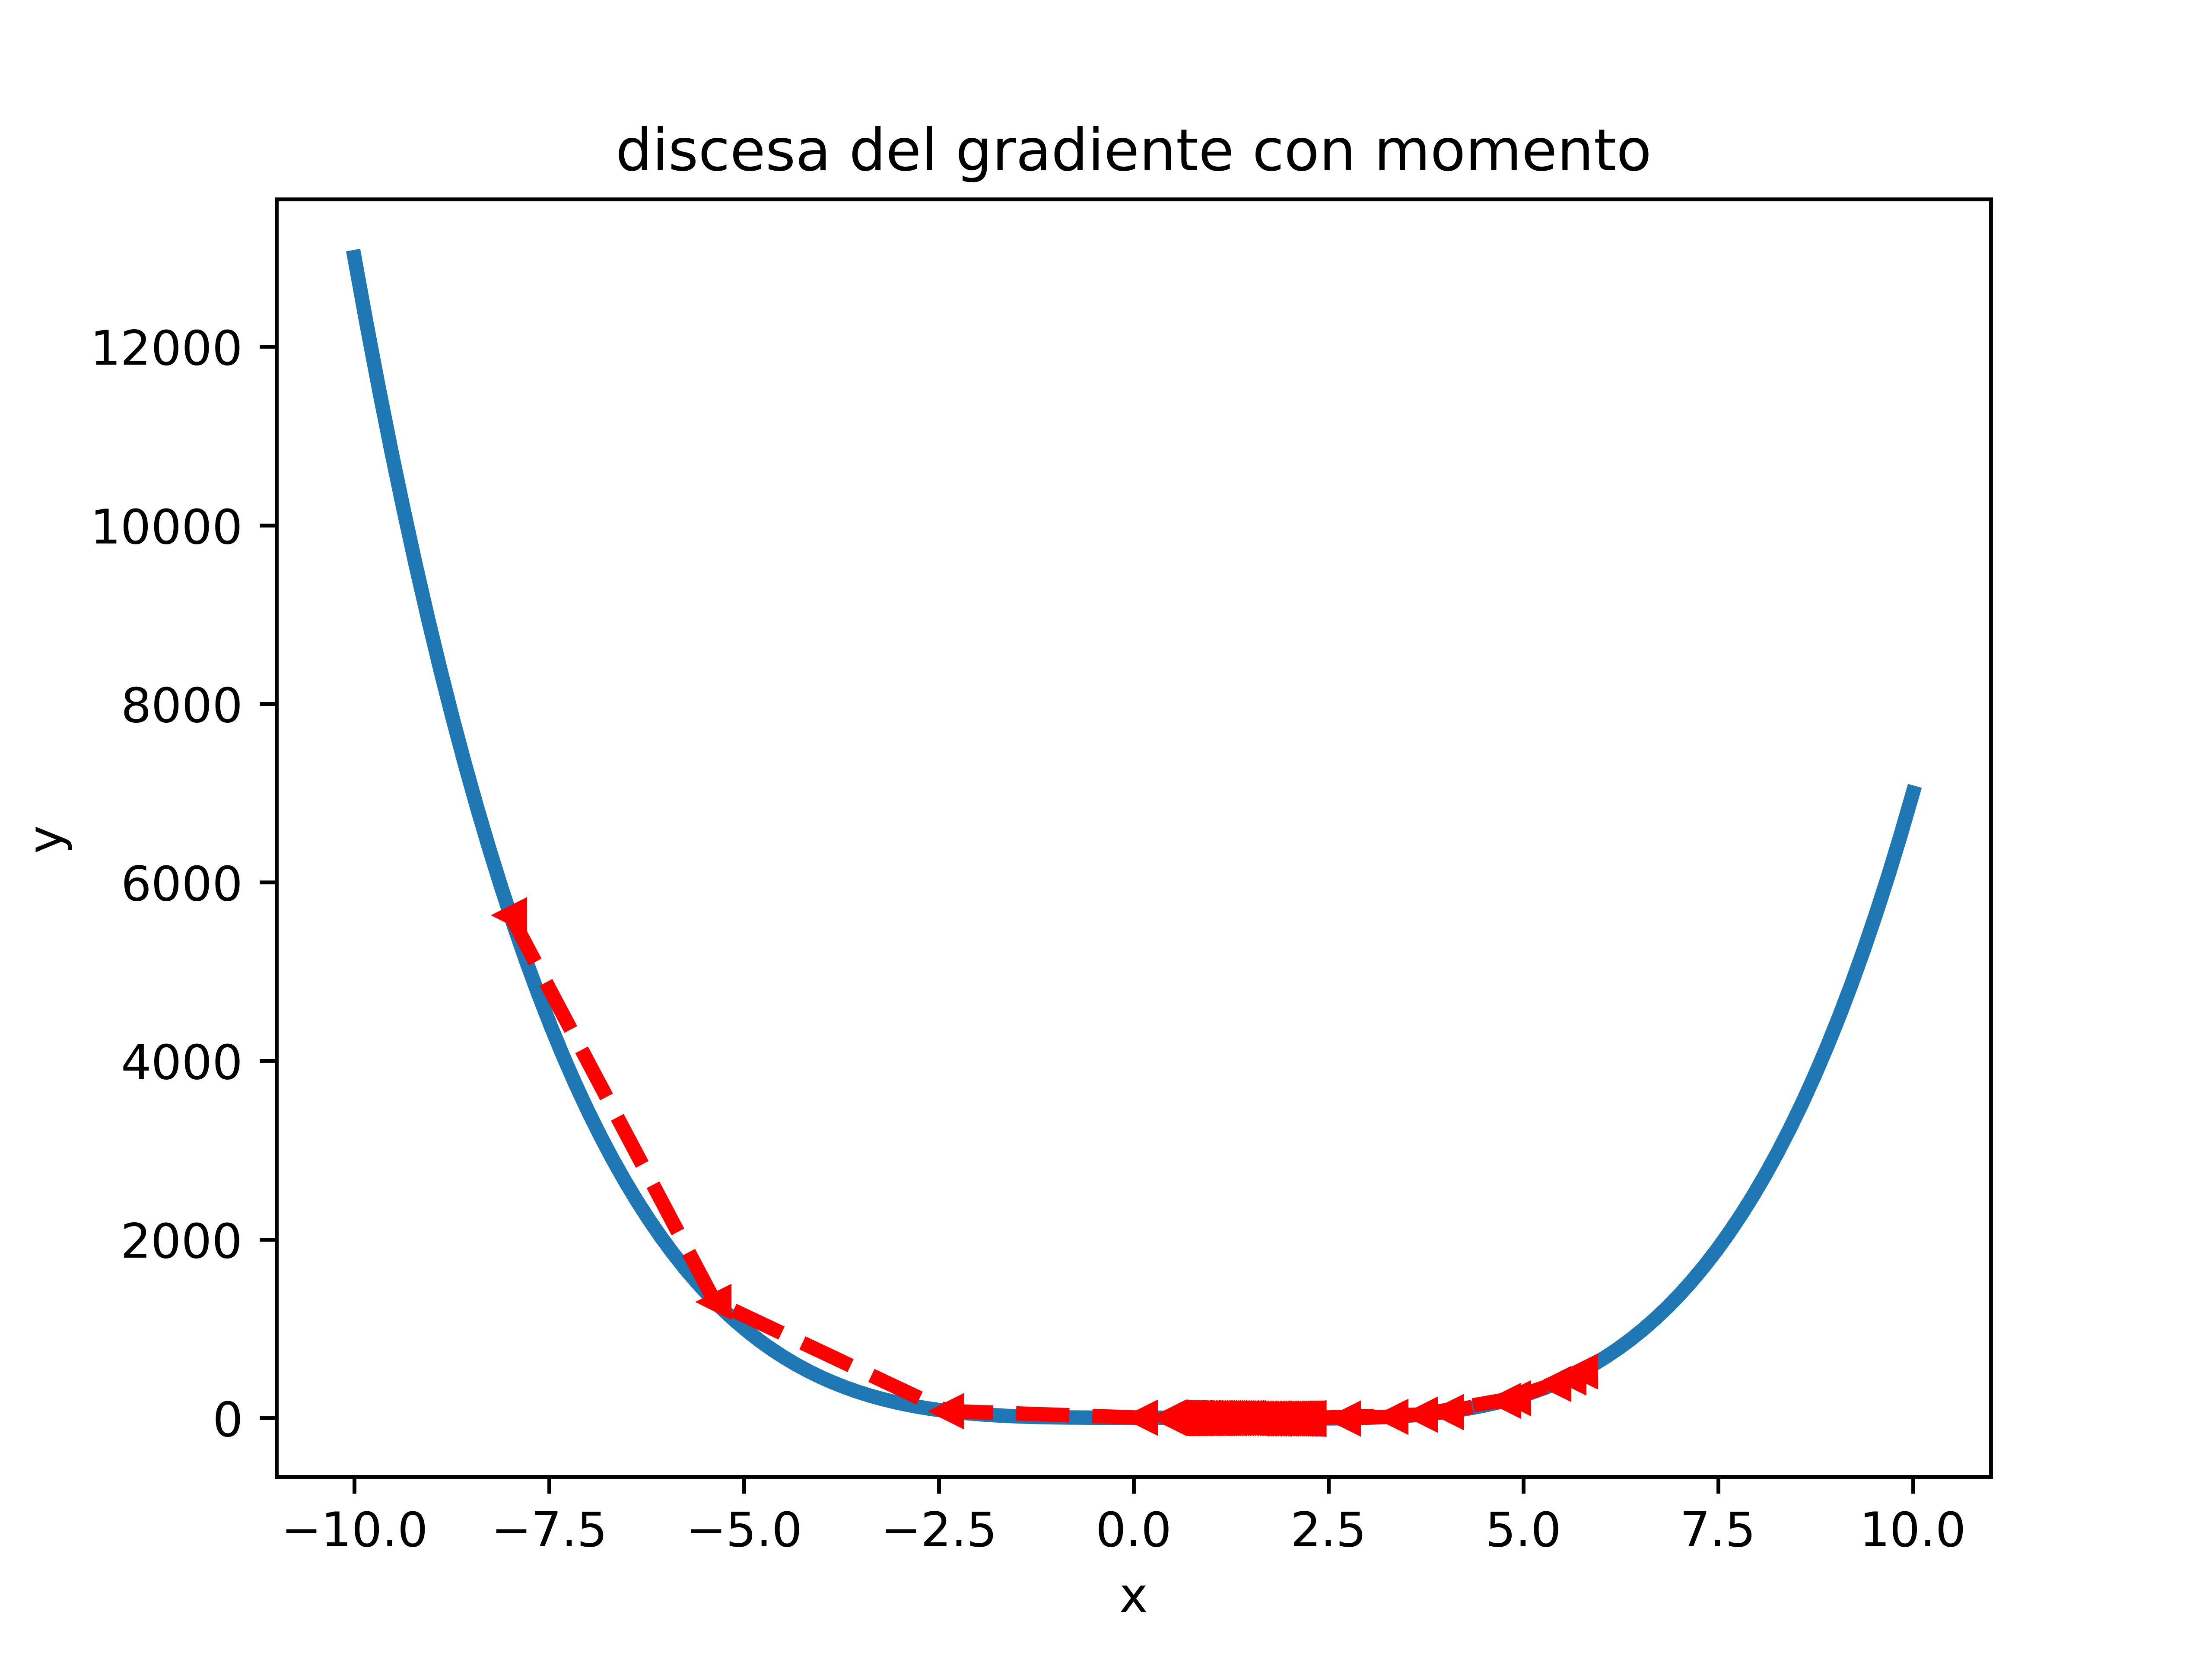
\includegraphics[width=1\textwidth]{images/momentum.png}
   \end{subfigure} 
   \begin{subfigure}{.49\textwidth}
    \centering
    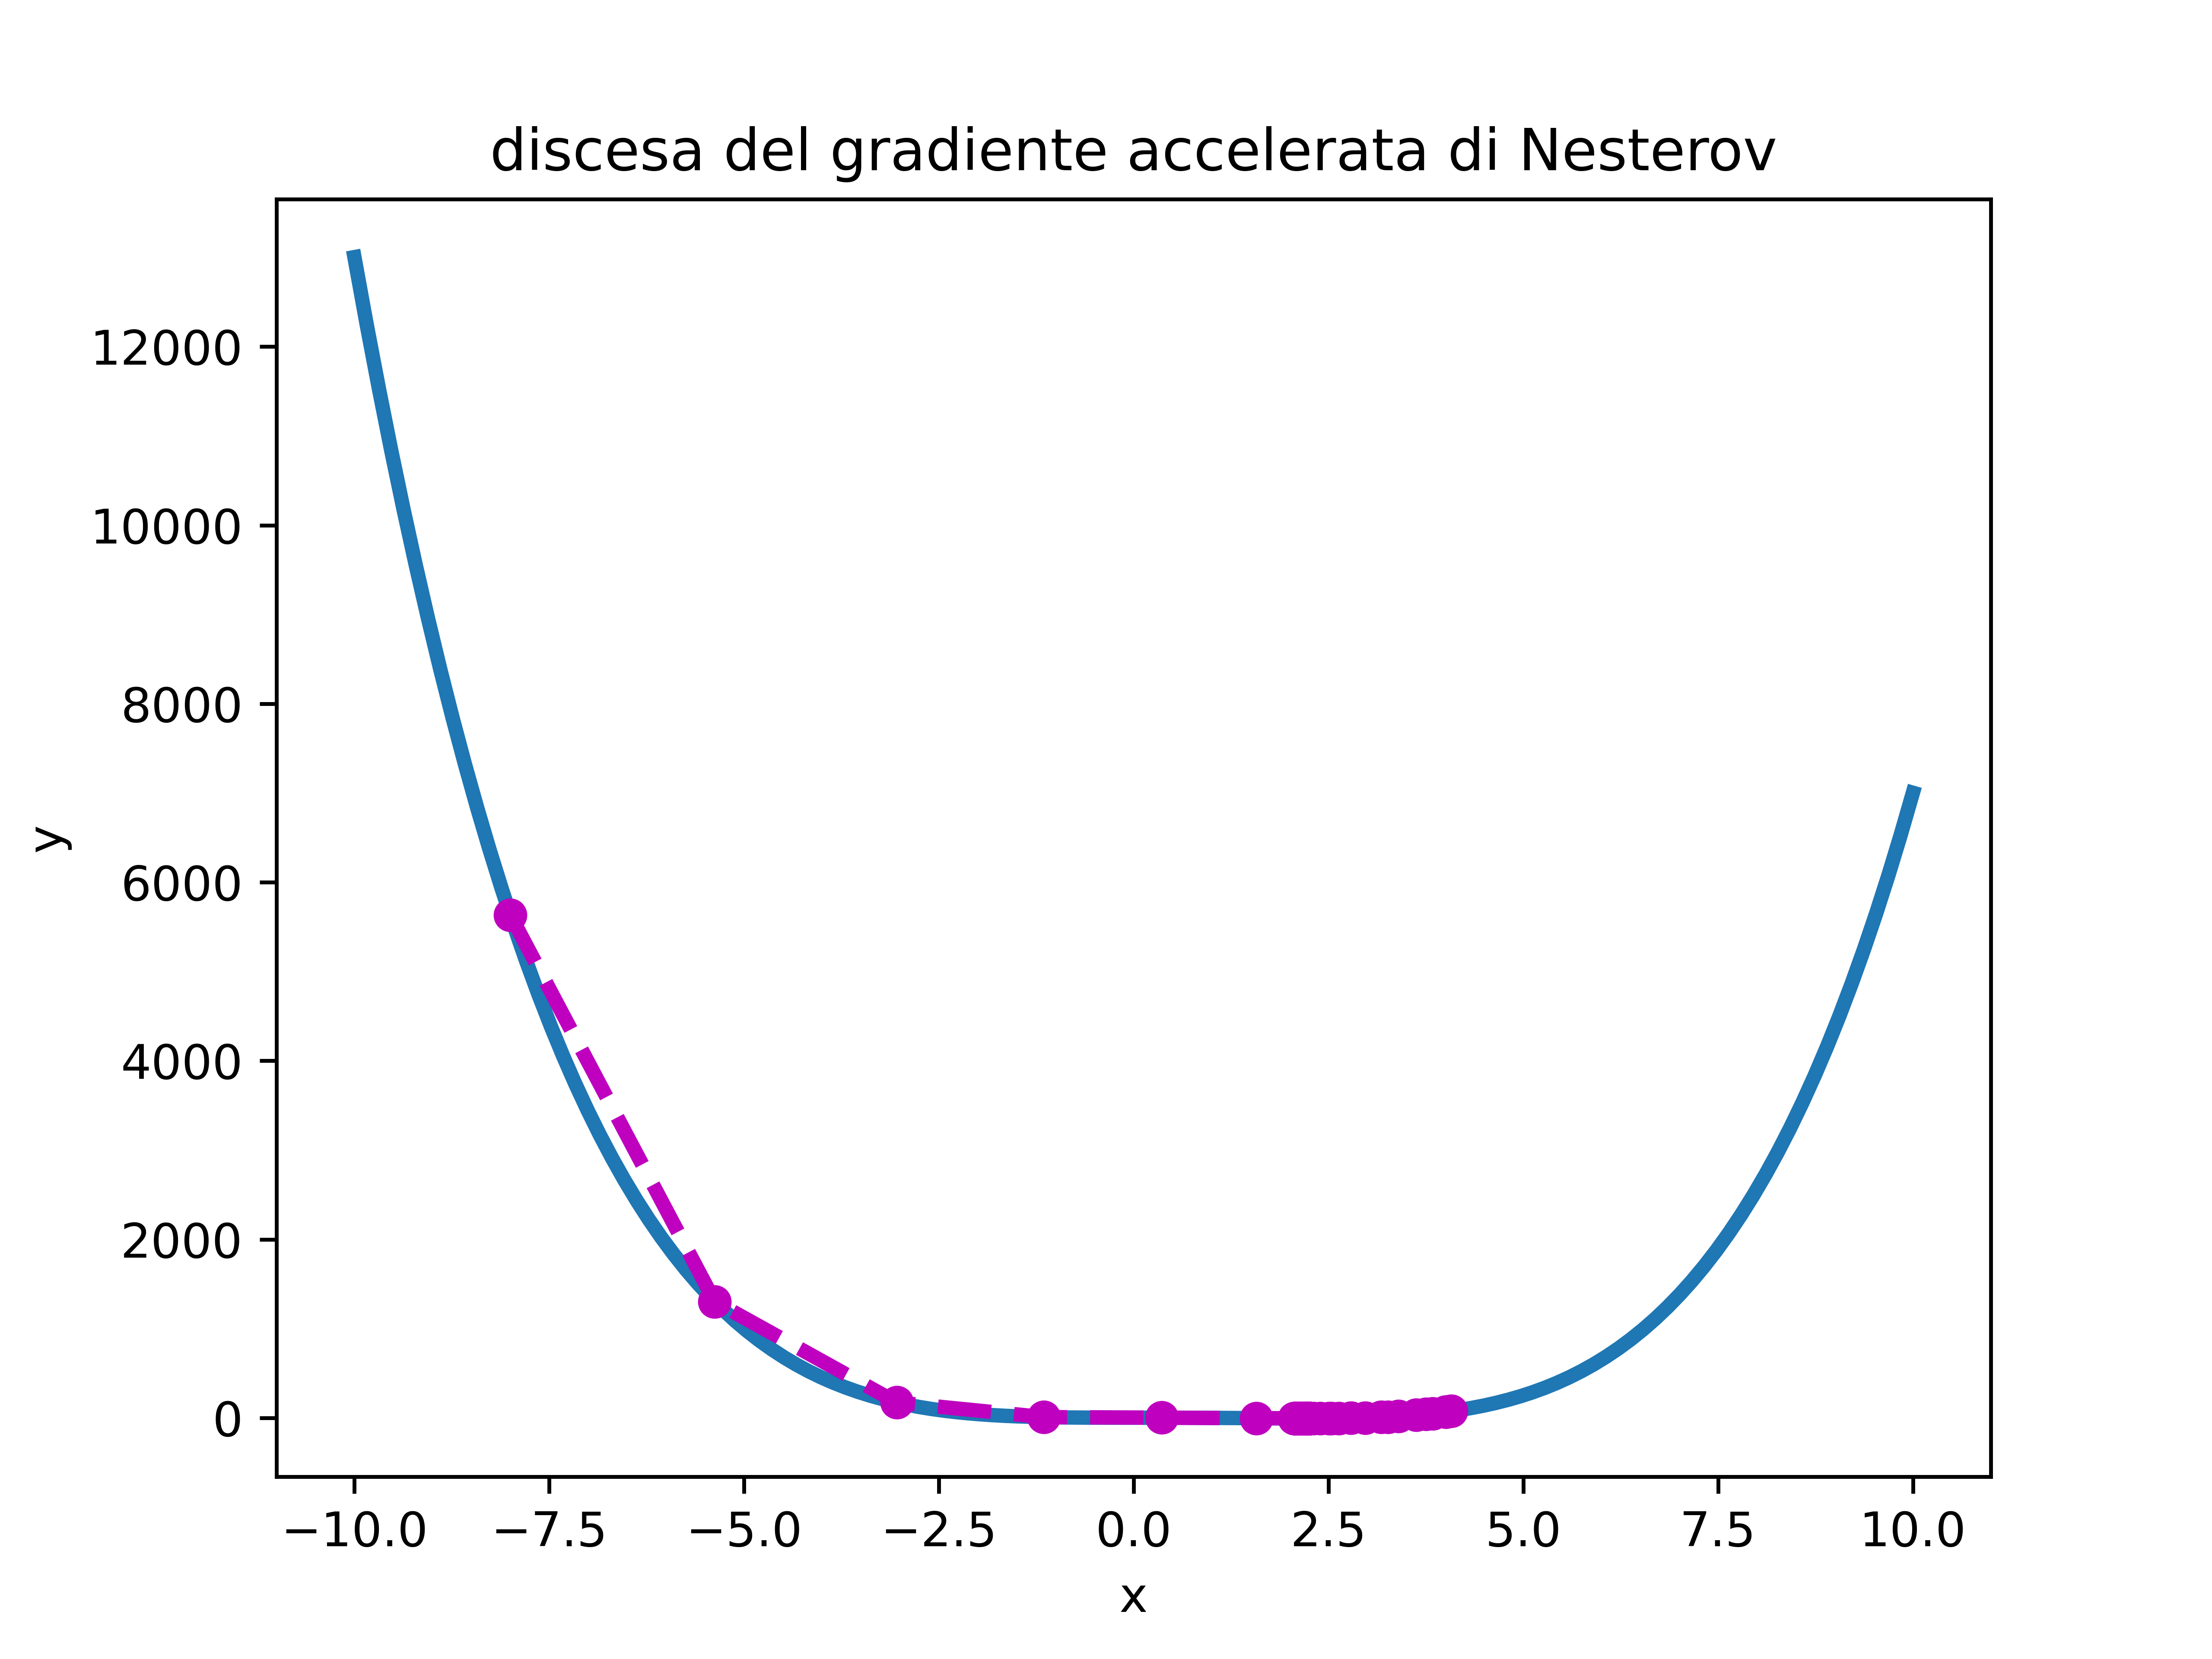
\includegraphics[width=1\textwidth]{images/nesterov.png}
\end{subfigure} 
   \caption{\emph{Tre grafici della funzione $f(x)$, tracciate su queste le traiettorie corrispondenti ai diversi algoritmi implementati, con tasso di apprendimento $\alpha = 0.001$, momentum parameter $\gamma = 0.8$ e posizione iniziale $x_0 = -8$.
   Osservare che mentre il primo algoritmo non superano il punto di sella, i due algoritmi più sofisticati lo sorpassano, e oscillano intorno al punto di minimo fino a raggiungerlo.}}
   \label{fig:confronto_algoritmi}
\end{figure}

L'implementazione dei vari metodi di discesa del gradiente è riportata sotto:

%-----codice python-----
\begin{lstlisting}[language = Python]
learning_rate = 0.001
momentum_parameter = 0.8
iteration_number = 10000
initial_pos = -8
initial_speed = 0

#gradient descent method
pos_grad = np.zeros(iteration_number+1)

#gradient descent with momentum method
pos_mom = np.zeros(iteration_number+1)
speed_mom = np.zeros(iteration_number+1)

#Nesterov method
pos_nesterov = np.zeros(iteration_number+1)
speed_nesterov = np.zeros(iteration_number+1)

#setting the initial position and speeds
pos_grad[0] = initial_pos

pos_mom[0] = initial_pos
speed_mom[0] = initial_speed

pos_nesterov[0] = initial_pos
speed_nesterov[0] = initial_speed

#function definitions
def gradient(pos):
    return 4*(pos**3) - 9*(pos**2)

def update_grad(pos, learning_rate):
    pos -= learning_rate * gradient(pos)
    return pos

def update_mom(pos, speed, learning_rate, momentum_parameter):
    speed = speed*momentum_parameter + learning_rate*gradient(pos)
    pos -= speed
    return (pos, speed)
    
def update_nesterov(pos, speed, learning_rate, momentum_parameter):
    speed = speed*momentum_parameter + learning_rate*gradient(pos-momentum_parameter*speed)
    pos -= speed
    return (pos, speed)

#booleans to indicate if it has found the minima:
reached_destination_grad = False
reached_destination_mom = False
reached_destination_nesterov = False

#update loop
for i in range(iteration_number):
    pos_grad[i+1] = update_grad(pos_grad[i], learning_rate)
    pos_mom[i+1], speed_mom[i+1] = update_mom(pos_mom[i], speed_mom[i], learning_rate, momentum_parameter)
    pos_nesterov[i+1], speed_nesterov[i+1] = update_nesterov(pos_nesterov[i], speed_nesterov[i], learning_rate, momentum_parameter)

    if not reached_destination_grad:
        if np.isclose(pos_grad[i+1], 9./4., atol=0.01) and np.isclose(pos_grad[i], 9./4., atol=0.01):
            print("classical gradient descent has reached global minima in ", i, "iterations")
            reached_destination_grad = True
        if np.isclose(pos_grad[i+1], 0., atol=0.01) and np.isclose(pos_grad[i], 0., atol=0.01):
            print("classical gradient descent has reached saddle point in ", i, "iterations")
            reached_destination_grad = True

    if not reached_destination_mom:
        if np.isclose(pos_mom[i+1], 9./4., atol=0.01) and np.isclose(pos_mom[i], 9./4., atol=0.01):
            print("gradient descent with momentum has reached global minima in ", i, "iterations")
            reached_destination_mom = True
        if np.isclose(pos_mom[i+1], 0., atol=0.01) and np.isclose(pos_mom[i], 0., atol=0.01):
            print("gradient descent with momentum has reached saddle point in ", i, "iterations")
            reached_destination_mom = True

    if not reached_destination_nesterov:
        if np.isclose(pos_nesterov[i+1], 9./4., atol=0.01) and np.isclose(pos_nesterov[i], 9./4., atol=0.01):
            print("nesterov has reached global minima in ", i, "iterations")
            reached_destination_nesterov = True
        if np.isclose(pos_nesterov[i+1], 0., atol=0.01) and np.isclose(pos_nesterov[i], 0., atol=0.01):
            print("nesterov has reached saddle point in ", i, "iterations")
            reached_destination_nesterov = True



#plotting
def overlay_trajectory(ax, xs, label, color='k', lw=2):
    ys = xs**4-3*xs**3+2
    ax.plot(xs,ys, color, label=label,lw=lw)
    return ax

fig1, ax1 = plt.subplots()
fig2, ax2 = plt.subplots()
fig3, ax3 = plt.subplots()

x = np.linspace(-10, 10, 128)
y = x**4 -3*x**3 +2

ax1.plot(x,y, lw= 3)
ax1.set_xlabel('x')
ax1.set_ylabel('y')
ax1.set_title("discesa del gradiente")

ax2.plot(x,y, lw= 3)
ax2.set_xlabel('x')
ax2.set_ylabel('y')
ax2.set_title("discesa del gradiente con momento")

ax3.plot(x,y,  lw= 3)
ax3.set_xlabel('x')
ax3.set_ylabel('y')
ax3.set_title("discesa del gradiente accelerata di Nesterov")

overlay_trajectory(ax1,pos_grad,'gradient','g--*', lw=3)
overlay_trajectory(ax2,pos_mom,'momentum','r--<', lw=3)
overlay_trajectory(ax3,pos_nesterov,'nesterov','m--o', lw=3)
\end{lstlisting}

\end{document}